\documentclass[tikz]{standalone}


\usepackage{graphicx}
\usepackage{pxfonts}
\usepackage{textcomp}
\newcommand{\figf}{\normalsize\sffamily\bfseries}



\begin{document}
\sffamily\scriptsize

\begin{tikzpicture}[anchor = north west]

	\clip (0,0) rectangle +(18,-19.7);

	\node at (0.7,-0.2) {\includegraphics{../plots/panelA.pdf}};
	\node at (0,0) {\figf A};
	\node at (4.5,0) {\figf B};

	\begin{scope}[yshift=-5cm]
	\begin{scope}
		\node at (0,0) {\includegraphics{../plots/panelB.pdf}};
		\node at (0,0) {\figf C};
		\node at (12.7,0) {\figf E};
		\node at (0,-3.7) {\figf D};
		\node at (12.7,-3.7) {\figf F};
	\end{scope}
	
	\begin{scope}[yshift=-7.5cm]
	
		\node at (1.7,-0.3) {Lm-RT (0h at 37\textcelsius): 75\% motile};
		\node at (7,-0.3) {Lm-RT (2h at 37\textcelsius): 79\% motile};
		\node at (12.3,-0.3) {Lm-RT (3h at 37\textcelsius): 56\% motile};
	
		\node[scale=0.55] at (1.7,-0.7) {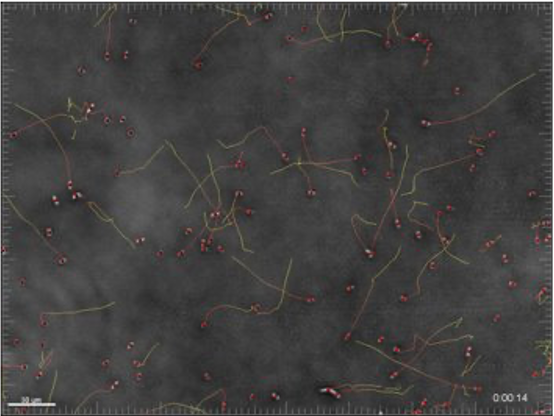
\includegraphics{../img/tracks-RT-0h.png}};
		\node[scale=0.55] at (7,-0.7) {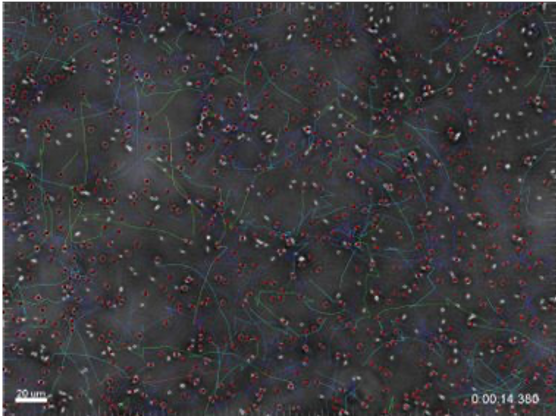
\includegraphics{../img/tracks-RT-2h.png}};
		\node[scale=0.55] at (12.3,-0.7) {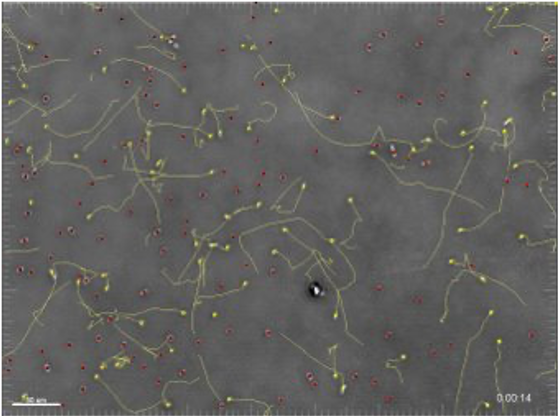
\includegraphics{../img/tracks-RT-3h.png}};
		
		\begin{scope}[yshift=-4cm]
		\node[scale=0.55] at (1.7,-0.7) {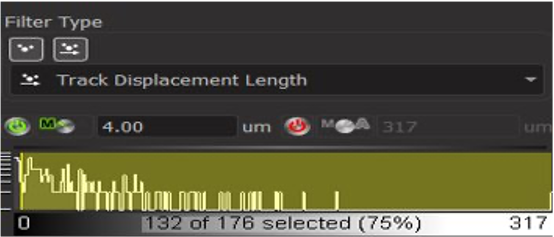
\includegraphics{../img/tracks-RT-0h-filter.png}};
		\node[scale=0.55] at (7,-0.7) {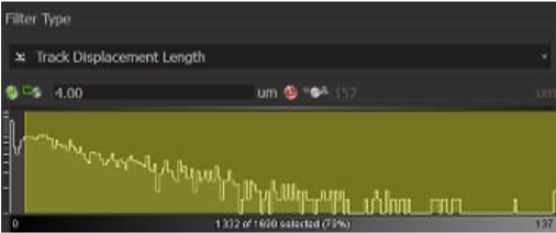
\includegraphics{../img/tracks-RT-2h-filter.png}};
		\node[scale=0.55] at (12.3,-0.7) {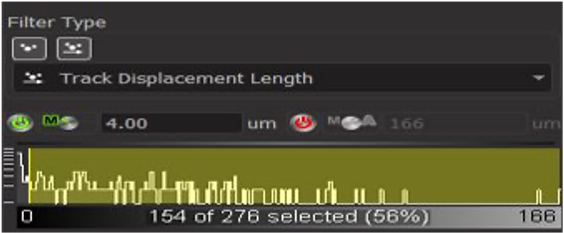
\includegraphics{../img/tracks-RT-3h-filter.png}};
		

		\end{scope}
		
		\node at (0,0) {\figf G};
	\end{scope}
	\end{scope}


	

\end{tikzpicture}

\end{document}